\documentclass[11pt]{article}
\usepackage[review]{acl}
\usepackage{times}
\usepackage{latexsym}
\usepackage[T1]{fontenc}
\usepackage[utf8]{inputenc}
\usepackage{microtype}
\usepackage{graphicx}
\usepackage{booktabs}
\usepackage{amsmath,amssymb}
\usepackage{array}
\usepackage{url}
\makeatletter
\let\inputtable\@@input
\makeatother
\newcommand{\bench}{\textsc{EduSkillBench}}
\newcommand{\noskill}{\textsc{No Skill}}
\newcommand{\withskill}{\textsc{With Skill}}
\title{EduSkillBench: Evaluating Procedural Skill Use\\in Educational Agents}
\author{Anonymous submission}
\begin{document}
\maketitle
\begin{abstract}
Reusable Skills can guide educational agents through teaching procedures,
but their availability does not establish that an agent uses them effectively.
We present \bench{}, a benchmark of 305 tasks across 14 educational Skill
families, linking teaching situations, procedural resources, execution
records, and artifact-level rubrics. Paired model evaluations show small,
mixed aggregate changes despite expected-package loading rates of
17.70--71.48\% across four native-access systems. Skill-level breakdowns and
paired traces expose both useful instructional operations and failures after
loading, including unavailable resources and incomplete delivery. A
28-task expert-adjudicated study covers all 14 families and finds that close
reference-relative scores can conceal larger component-score disagreements.
We further examine learning from 246 Skill-informed artifacts through
Qwen3-4B SFT and subsequent outcome-based reinforcement learning, alongside
an execution-cost pilot. \bench{} provides a connected evaluation of
procedural availability, observed use, and usable educational output.
\end{abstract}

\begin{figure*}[t]
\centering
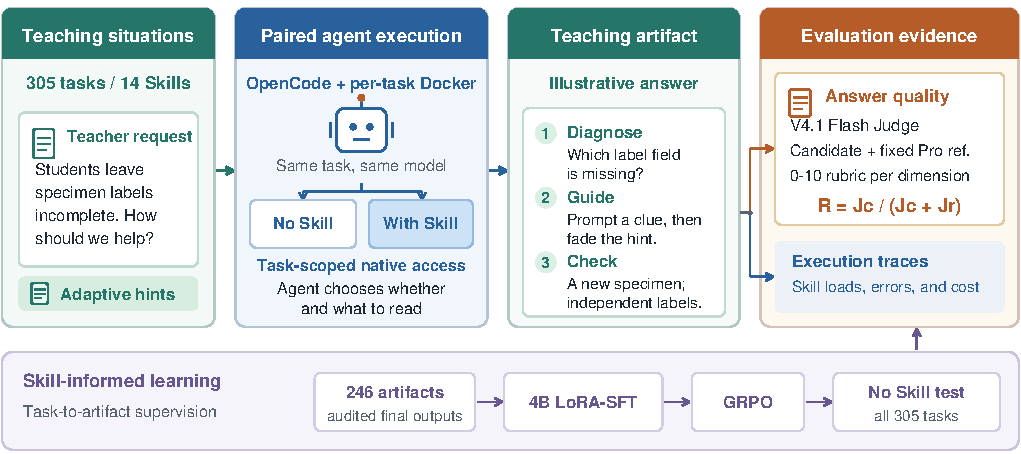
\includegraphics[width=\textwidth]{figures/framework_v4.pdf}
\caption{Overview of \bench{}. Teaching tasks bind procedural resources to
artifact requirements and rubric criteria. Paired native execution exposes a
task-matched Skill for autonomous access; a separate artifact-learning study
tests performance without Skill documents. Retained outputs support outcome,
access, and human--judge analyses. Rubrics and evaluation references are used
after generation. Exposure details are in Appendix~\ref{app:execution}.}
\label{fig:pipeline}
\end{figure*}
\section{Introduction}

Educational assistants must turn knowledge into instructional decisions: which
hint to offer after an unsuccessful attempt, what evidence would demonstrate
understanding, and how to organize practice within a limited timetable.
Producing a plausible explanation of a teaching method is easier than adapting
that method to a learner and delivering materials a teacher can use. This
distinction is central to pedagogical content knowledge and scaffolding
\citep{shulman1986,wood1976}, and remains relevant to language models:
MathTutorBench finds that subject-solving ability does not automatically
translate into effective tutoring \citep{mathtutorbench}.

Recent work addresses this gap through pedagogical instruction following and
explicit expert decisions \citep{learnlm,bridge}. Reusable \emph{Agent Skills}
offer a complementary approach: package a procedure, its templates, and
supporting resources so that an agent can consult them when needed
\citep{agentskills}. For example, an adaptive-hint package can connect evidence
of a student's difficulty to graduated assistance and a check for independent
understanding. Its educational value depends on whether the agent selects
applicable operations and completes them correctly. Merely making the document
available does not establish that connection.

Existing benchmarks provide complementary evidence. EduBench covers diverse
educational requests, while MathTutorBench and MRBench assess open-ended
tutoring behavior \citep{edubench,mathtutorbench,mrbench}. SkillsBench evaluates
procedural packages through paired agent runs and executable verification
\citep{skillsbench}. Open-ended teaching products introduce a further challenge:
a generated lesson, diagnostic question, or practice schedule may be fluent
and procedurally detailed yet infeasible or substantively incorrect. Measuring
Skill use in this setting requires linking a teaching task to its procedural
resource, the agent's actions, and the quality of the delivered product.

We introduce \bench{}, a unified benchmark of 305 tasks across 14 educational
Skill families. Each task binds a teaching situation, a designated Skill, and
applicable rubric criteria. Paired \noskill{} and \withskill{} evaluations
compare delivered outcomes with and without procedural support; native execution records
show whether agents actually load it. Reference-conditioned judgments assess
the delivered text provided to the evaluator, while a 28-task expert-adjudicated sample checks
how those judgments behave across the 14 families. A complementary Qwen3-4B
study examines learning from Skill-informed artifacts through supervised
fine-tuning (SFT) and subsequent outcome-based reinforcement learning.

The analysis reveals a gap between access and useful delivery. Across four
native-access models, expected-package loading ranges from 17.70\% to 71.48\%,
but aggregate With--No changes remain between $-1.19$ and $+0.50$ score points.
Family breakdowns and paired cases locate more explicit teaching operations,
resource failures, and incomplete deliverables behind those averages.
Human-adjudicated scores further show that close reference-relative scores can
coexist with substantial differences in their underlying quality components.
These findings motivate evaluating procedural support at both the execution
and artifact levels.

Our contributions are threefold: (1) a 305-task educational benchmark linking
14 reusable Skills to explicit output requirements and rubrics; (2) paired
model evaluations with family-level outcomes, observable Skill access, and
trace-based explanations; and (3) complementary studies of artifact learning,
expert-adjudicated evaluation, and execution cost. Together, they make the
path from procedural guidance to educational work empirically inspectable.

\section{Related Work}
\label{sec:related}

\paragraph{Educational capability and teaching decisions.}
Educational evaluation increasingly distinguishes knowing an answer from
helping a learner. MathTutorBench evaluates open-ended pedagogical abilities,
and MRBench organizes the assessment of remediation responses
\citep{mathtutorbench,mrbench}. EduBench extends coverage to diverse teacher-
and student-facing scenarios \citep{edubench}; EduIllustrate evaluates the
quality of instructional products across several subjects and dimensions
\citep{eduillustrate}. On the intervention side, Bridge models expert decisions
about mistakes and remediation, LearnLM targets pedagogical instruction
following, and Tutor CoPilot studies expert-inspired assistance in live
tutoring \citep{bridge,learnlm,tutorcopilot}. \bench{} focuses on a different
unit of evaluation: a teaching task linked to a reusable procedure and the
agent execution that produces its instructional artifact. Artifact quality
does not by itself establish student learning gains.

\paragraph{External Skills and learned procedures.}
ReAct connects actions to observations, while Voyager retains reusable
programs in a Skill library \citep{yao2023react,wang2024voyager}. Agent Skills
provide a document-and-resource interface for procedural guidance
\citep{agentskills}; SkillsBench tests curated packages through paired task
executions \citep{skillsbench}. We examine autonomous use of a task-matched
educational candidate, where a correct package may be available but unread or
incompletely applied. Parameter learning poses a separate question.
SkillGym trains from successful Skill-enabled interactions, and SKILL0 studies
progressive withdrawal of Skill context during reinforcement learning
\citep{skillgym,skillzero}. Distilling Step-by-Step distinguishes rationale
from output supervision, and AgentInstruct synthesizes teaching data through
agentic flows \citep{hsieh2023distilling,mitra2024agentinstruct}. Our small-model
study uses final teaching artifacts for SFT and outcome-based GRPO
\citep{deepseekmath}; its learned target differs from supervising tool calls
or full environment interactions.

\paragraph{Evaluation of open-ended artifacts.}
LLM judges scale response evaluation but can introduce systematic biases
\citep{zheng2023judging}. G-Eval and Prometheus use explicit criteria and
structured scoring, while JudgeBench emphasizes objective error detection
\citep{geval,prometheus,judgebench}. We adapt QUEST's joint candidate/reference
comparison \citep{quest} and retain both component scores. Following the
diagnostic role of breakdowns in EduIllustrate \citep{eduillustrate}, we examine
agreement separately across educational Skill families and at the component
and relative-score levels. This establishes where an evaluator agrees with
reviewers, rather than treating a single aggregate as universal validation.

\section{EduSkillBench}
\label{sec:benchmark}
\label{sec:framework}

\subsection{Task Definition and Construction}
Given a teaching situation and request, an agent produces an instructional
artifact: for example, a lesson plan, diagnostic question, support sequence,
project brief, or practice schedule. Successful work requires interpreting
the available evidence, choosing appropriate teaching operations, and
delivering a correct, feasible product. Each task binds the situation and
request to a designated Skill and a fixed set of applicable rubric dimensions.
The Skill supplies reusable procedural support; it is not a reference answer.

The unified inventory contains 305 tasks across 14 Skills. It combines 263
Chinese teaching scenarios adapted from 30 documents in the archived
\texttt{edu\_scene\_66} collection with 42 constructed English tasks, three
per Skill. The source scenarios cover nine families; the constructed tasks
extend coverage to all 14. Versioned revisions repair identified mismatches
between questions, contexts, and criteria. Each constructed task specifies
the requested artifact and constraints at one of three nominal difficulty
levels. These levels organize construction, rather than constitute a
calibrated proficiency scale. All 305 tasks receive equal weight in the
primary result.

The packages are drawn from public educational Skill collections
\citep{educationagentskills,teachingskills}. They cover planning and alignment,
diagnostic questioning, adaptive support, learner participation, and practice
over time. Family sizes range from three to 157 tasks; lesson building
accounts for 51.48\% of the inventory. Figure~\ref{fig:skill-breakdown} reports
all family counts, and Appendix~\ref{app:inventory} preserves the full task
and training distribution.

\paragraph{An example of procedure fit.}
One task asks how to help a fourth-grade pupil label rock specimens independently
when labels are crooked or omit names and collection sites. Its adaptive-hint
Skill connects diagnosis to graduated assistance and an independence check.
The response must provide usable prompts and checks suited to this obstacle;
reproducing an entire teaching template is unnecessary. The applicable rubric
covers accuracy, scaffolding, guidance, age suitability, and safety. This
task--procedure--criterion binding makes the intended support observable.
It does not provide an answer key for every new example the agent may invent.

\subsection{Paired Agent Execution}
\label{sec:protocol}
The native protocol uses an isolated Docker workspace for each task and
OpenCode 1.18.11 with an educational single-turn agent instruction.
\noskill{} exposes no educational package. \withskill{} makes the designated
task-matched package available through the native Skill interface. The agent
decides whether to load it, inspect resources, and apply particular operations.
This measures autonomous use of the available candidate; it does not test
retrieval across all 14 Skills. Rubrics and evaluation references are withheld
from generation.

The agent deadline is 600 seconds, with a 480-second provider timeout and a
10,000-token output cap per model call. Multiple calls may occur within a
trajectory. Paired runs retain the requested artifact, available tool records,
and execution status. There is one accepted outcome per model--task--condition,
and completed answers are reused when only judging needs recovery.
Exact model settings and the retained GLM-5.3 exposure inventory are documented
in Appendix~\ref{app:execution}.

\subsection{Reference-Conditioned Artifact Evaluation}
\label{sec:judge}
DeepSeek V4.1 Flash jointly evaluates each candidate and the task's saved
DeepSeek V4 Pro \noskill{} answer. The two texts appear as anonymous A/B
responses, with hash-assigned order, the task, and its applicable rubric.
The evaluator sees the retained delivery text; files absent from that input
are not automatically inspected.
Following the comparison mechanism of QUEST \citep{quest}, both receive
dimension scores $s_{x,i,d}\in[0,10]$. We compute
\begin{align}
J_{x,i}&=\frac{1}{10D_i}\sum_{d=1}^{D_i}s_{x,i,d},\\
R_i&=\frac{J_{c,i}}{J_{c,i}+J_{r,i}},\qquad
S=\frac{100}{305}\sum_{i=1}^{305}R_i,
\label{eq:refscore}
\end{align}
where $D_i$ is the number of applicable dimensions and $c,r$ denote candidate
and reference. All tasks use this equal-weight rule, regardless of their
construction origin. $R_i=0.5$ means parity with the reference under that
judgment, not 50\% accuracy. Pro's reference-self condition receives 0.5;
execution failures receive zero in the fixed 305-task denominator. A pair
with both components zero is unresolved; none remain in the reported archive.

The judge checks correctness, consistency, feasibility, and task constraints;
scores of at least 9 require response evidence. Substantive errors reduce
relevant dimensions. Structural validators check coverage, evidence bindings,
and score ranges. The reference is a comparison anchor, not a gold answer:
generated scientific examples have no independent computational oracle.
We therefore retain both $J$ components and compare judgments with expert
adjudication in Section~\ref{sec:human-summary}. A stable ratio can conceal
shared changes in candidate and reference scores.

\section{Experimental Results}
\label{sec:experiments}
\subsection{Experimental Setup}
We evaluate GLM-5.3, GLM-5.3 Flash, DeepSeek V4.1 Flash, DeepSeek V4 Pro,
and Doubao Seed 2.1 Pro on the same 305 tasks in both conditions. All 3,050
cells have a resolved score or an explicit execution-failure status. The
native-access analysis covers the latter four systems; the archived GLM-5.3
row is retained in outcome comparisons, with its exposure provenance recorded
in Appendix~\ref{app:execution}. Qwen3-4B and its SFT/GRPO adapters form a
separate learning comparison without external Skills.

The experiments ask three connected questions: how outcomes vary across
Skills, how observed access relates to the resulting artifact, and whether
Skill-informed demonstrations support performance without external resources.
Expert-adjudicated judgments and cost measurements assess the reliability
and practical requirements of these comparisons. All reported score changes
are on the 0--100 reference-relative scale of Equation~\ref{eq:refscore}.

\subsection{Overall Performance and Skill Breakdown}
\label{sec:results}
\label{sec:skill-breakdown}

\begin{table*}[t]
\centering\small
\begin{tabular}{lrrrr}
\toprule
Model & No Skill & With Skill & $\Delta$ (points) & Failures (No/With)\\
\midrule
\inputtable{tables/combined_main.tex}
\bottomrule
\end{tabular}
\caption{Reference-relative scores on the unified 305-task inventory. All
tasks remain in each denominator; execution failures contribute zero. Pro No
Skill supplies the fixed references and is assigned the self-comparison value
50.00. GLM-5.3 is the retained augmentation result described in
Appendix~\ref{app:execution}. Differences use unrounded values.}
\label{tab:main}
\end{table*}

\paragraph{Procedural availability produces selective gains.}
Table~\ref{tab:main} covers 3,050 model--task--condition cells: 2,725
accepted judgments, 305 reference-self comparisons, and 20 execution failures.
GLM-5.3, GLM Flash, and Doubao improve by 0.45, 0.41, and 0.50 points with
Skill availability, whereas DeepSeek Flash and Pro decline by 1.19 and
0.25 points. The small aggregate changes motivate examining which educational
procedures help, whether agents access them, and what they ultimately deliver.
They do not support a uniform benefit from adding procedural resources.

\begin{figure*}[t]
\centering
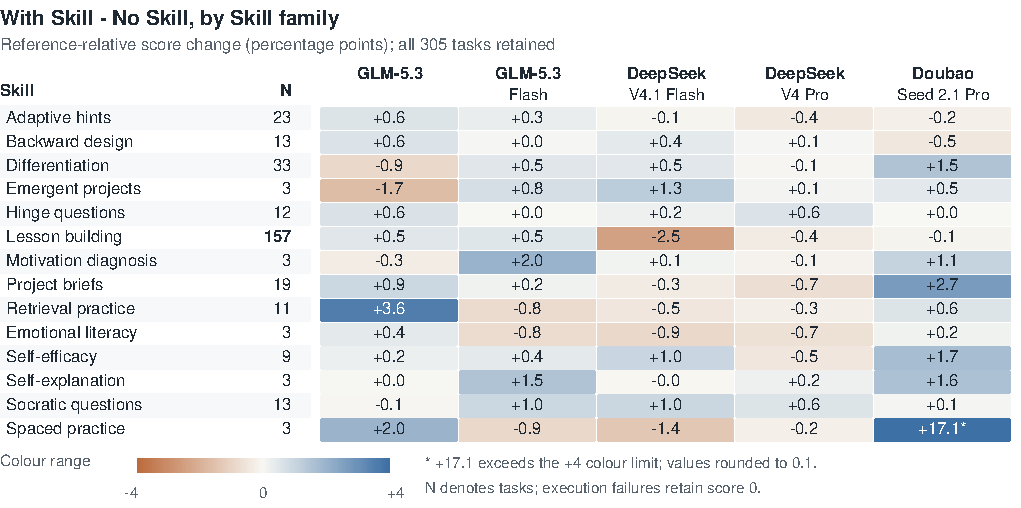
\includegraphics[width=\textwidth]{figures/skill_delta_v4.pdf}
\caption{With--No score differences for all five models across the 14 Skills.
Each cell retains all tasks in its family, including failures; $n$ gives the
family size. Color saturates at $\pm4$ points; labels show rounded
differences. Complete means and failure counts appear in
Appendix~\ref{app:inventory}.}
\label{fig:skill-breakdown}
\end{figure*}

\paragraph{Different procedures reveal different strengths.}
Figure~\ref{fig:skill-breakdown} groups the same accepted scores by designated
Skill, without changing the judge or task membership. GLM-5.3, GLM Flash,
DeepSeek Flash, Pro, and Doubao have positive differences on 10, 11, 7, 5,
and 11 of 14 families. For example, GLM Flash gains 0.95 points on Socratic
questioning but loses 0.81 on retrieval practice. DeepSeek Flash gains 1.01
on self-efficacy support and 0.98 on Socratic questioning, yet loses 2.49 on
lesson building. These contrasts locate procedure-specific opportunities
that the overall mean conceals.

\paragraph{Coverage and completion explain part of the variation.}
Lesson building contributes 157/305 tasks (51.48\%), while five families
contain three tasks each. Its decline contributes $-1.28$ points to DeepSeek
Flash's overall $-1.19$ change. Equal weighting of the 14 families instead
gives changes of $+0.47$, $+0.34$, $-0.09$, $-0.13$, and $+1.87$ points
in the model order above; this diagnostic describes coverage sensitivity,
while the task-weighted mean remains primary.

Completion also matters. Doubao's spaced-practice gain is $+17.06$ on three
tasks, including one failed No Skill execution; the two pairs completed in
both conditions differ by only $+0.59$. Across all common-valid pairs, the
four native-access models change by $+0.25$, $-0.54$, $-0.09$, and $+0.36$
points, respectively. DeepSeek Flash's decline therefore persists after
conditioning on completion. Appendix~\ref{app:inventory} supplies family
denominators and failure diagnostics. These single-run differences describe
the retained executions; they do not establish significance across model
or judge resampling.

\subsection{From Skill Access to Usable Teaching Artifacts}
\label{sec:access}
\label{sec:cases}

The native interface exposes the task's designated educational package;
the agent decides whether to load it. We count a completed call naming that
package, requiring returned content for locally available raw traces and
using completed-call summaries where those are the retained evidence.
Missing captures remain unknown. GLM-5.3 is excluded from this access
analysis because its retained answers span two exposure modes
(Appendix~\ref{app:execution}).

\begin{figure*}[t]
\centering
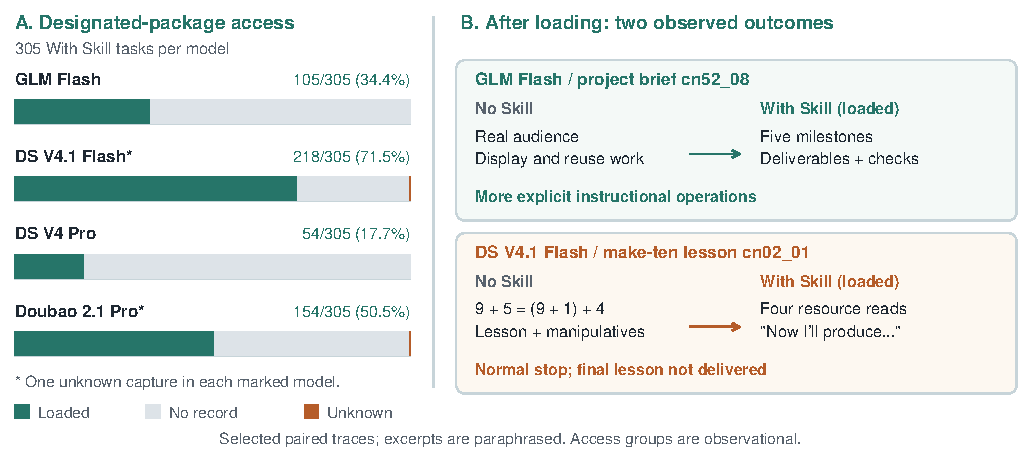
\includegraphics[width=\textwidth]{figures/access_artifacts_v41.pdf}
\caption{From package availability to teaching artifacts. Left: observed
access among 305 With tasks per model; unknown captures are separate from
no recorded access. Right: paraphrased paired artifacts show explicit project
milestones after loading, but a lesson that ends as a promise rather than a
deliverable. Cases illustrate mechanisms, not prevalence or a causal effect
of loading. Full subgroup results appear in Appendix~\ref{app:inventory}.}
\label{fig:access-artifacts}
\end{figure*}

\paragraph{Availability does not guarantee access.}
Figure~\ref{fig:access-artifacts} records 531 loads over 1,220 With tasks, ranging
from Pro's 17.70\% to DeepSeek Flash's 71.48\%. Every recorded educational
load names the designated package. With one task-scoped educational candidate,
this measures the decision to access relevant guidance; it does not test
retrieval among all 14 Skills. Loaded common-valid groups improve for GLM
Flash, Pro, and Doubao, but decline for DeepSeek Flash. Since agents choose
whether to load and the resulting groups differ in task composition, these
associations do not identify a causal loading effect.

\paragraph{A useful procedure makes classroom operations explicit.}
In GLM Flash's project-brief task \texttt{cn52\_08}, the teacher has no
budget or laboratory and wants student projects with a real audience. Both
answers identify meaningful uses for the work. After loading the package,
the With answer additionally organizes five milestones, stage-specific
deliverables, explicit instruction, and completion checkpoints. This is
observable procedural uptake beyond mentioning the Skill. Judged candidate quality
$J$ rises from 0.856 to 0.912, although the reference component also falls
from 0.918 to 0.806; the resulting $+4.83$ relative-score change therefore
cannot be assigned entirely to the candidate's improvement.

\paragraph{Successful access can still end without a deliverable.}
For DeepSeek Flash's lesson-building task \texttt{cn02\_01}, No Skill
provides a concrete make-ten lesson with manipulatives and fallback materials.
With Skill loads the package and four resources, but terminates with a
promise to produce materials instead of the lesson itself. The answer has
a normal stop and a zero candidate component. More broadly, DeepSeek Flash
has 60 failed supporting-file reads over 49 tasks despite successful main
package loads. These records distinguish access, resource execution, and
final delivery. Our 32 exported paired cases connect those stages to actual
teaching products; they were selected diagnostically and do not estimate
failure prevalence (Appendix~\ref{app:inventory}).

\subsection{Learning to Produce Artifacts Without External Skills}
\label{sec:internalization}

We further ask whether Skill-informed demonstrations can improve a small
model when the procedural documents are absent at inference. Inspired by
SkillGym's distinction between external assistance and parameter transfer
\citep{skillgym}, we compare Qwen3-4B-Instruct-2507, LoRA-SFT, and subsequent
outcome-based GRPO on the same 305 tasks under No Skill.

\paragraph{Teach decisions through complete artifacts.}
We decompose the 14 Skills into operations and evidence that should change
their application: repeated failed hints, for example, should trigger a
different response from an initial request for help. EduBench question seeds
are reconstructed around complete-product creation, changed learner evidence,
resource boundaries, and artifact repair. Screening and revision retain
246 demonstrations: 162 generated reference artifacts, 52 revised artifacts,
and 32 final answers from environment executions. Each student input contains
the task; the supervised target is its complete teaching artifact. Skill
documents and rubrics are omitted from student inputs. This supervision
targets educational decisions expressed in products, rather than native
tool-call trajectories.

SFT applies completion-only loss for one epoch, preserving all complete
targets within 8,192 tokens. GRPO starts from that adapter, samples eight
answers per training question, and runs 123 optimization steps. The training
judge assigns the equally weighted PASS fraction under the task rubric;
empty or truncated answers receive zero. This outcome reward differs from
the final reference-relative evaluation. Full recipes and provenance are
in Appendix~\ref{app:execution}.

\begin{table}[t]
\centering\small
\begin{tabular}{lrrr}
\toprule
Stage & No Skill & $\Delta_{\mathrm{Base}}$ & $\Delta_{\mathrm{prev}}$\\
\midrule
\inputtable{tables/internalization.tex}
\bottomrule
\end{tabular}
\caption{Reported 305-task No Skill aggregates for Qwen3-4B and its two
adapters. The latest per-task recovery archive remains to be reconciled
with this supplied aggregate version (Appendix~\ref{app:execution}).}
\label{tab:internalization}
\end{table}

The reported sequence is 41.56$\rightarrow$42.69$\rightarrow$43.04:
$+1.13$ points after SFT and another $+0.35$ after GRPO. This is a modest
descriptive improvement, not a demonstrated routing capability or a
significant effect. Training uses non-identical benchmark-derived variants,
so the comparison concerns related educational families rather than
unseen-family generalization. Updated adapter evaluations also recover
historical execution failures; item-level reconciliation is needed to
separate recovery and answer-quality contributions before finalizing the
learning claim.

\subsection{Human--Judge Agreement}
\label{sec:human-summary}

\begin{figure*}[t]
\centering
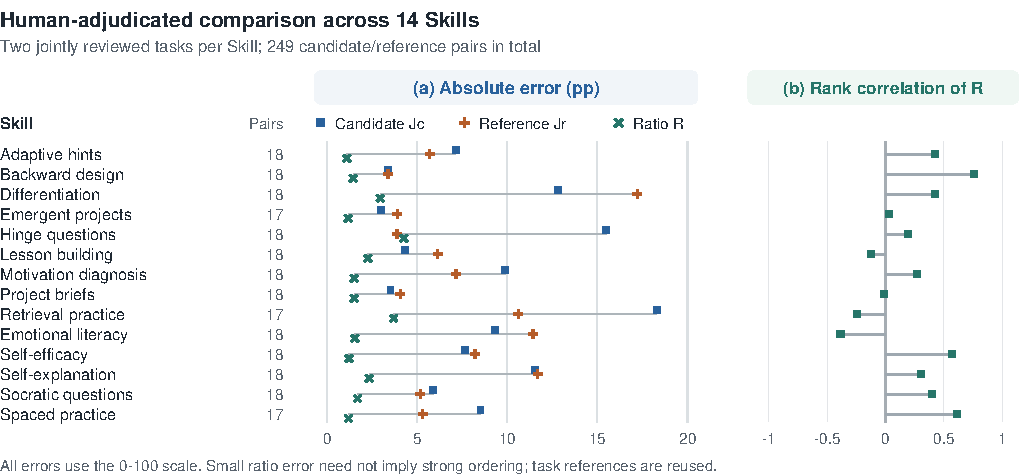
\includegraphics[width=\textwidth]{figures/human_review_v4.pdf}
\caption{Human--Judge comparison across 14 Skills: two reviewed tasks per
Skill and 249 substantive pairs. Left: candidate $J_c$, reference $J_r$,
and relative-score $R$ MAE (percentage points). Right: $R$ Spearman
correlation. References are reused within tasks; small ratio errors can
coexist with weak ordering agreement.}
\label{fig:human-breakdown}
\end{figure*}

\paragraph{Design.}
Two expert reviewers jointly adjudicated 28 tasks, two per Skill, covering
five models in both conditions. Excluding 28 reference-self and three
execution-failure controls leaves 249 candidate--reference pairs. Reviewers
use the same rubric and 0--10 scale, scoring each reference once.
Following \citet{eduillustrate}, we examine agreement by educational
dimension; here the breakdown follows 14 Skill families
(Appendix~\ref{app:human}).

\begin{table}[t]
\centering\small
\setlength{\tabcolsep}{5pt}
\begin{tabular}{lrrr}
\toprule
Score & MAE & Bias & $\rho$\\
\midrule
\inputtable{tables/full_ref_metrics.tex}
\bottomrule
\end{tabular}
\caption{249-pair agreement. MAE and human-minus-Judge bias are in
percentage points; $\rho$ is Spearman correlation.}
\label{tab:ref-human-metrics}
\end{table}

\paragraph{Score proximity and ranking differ.}
Table~\ref{tab:ref-human-metrics} shows a 1.99-point $R$ MAE, compared
with 8.61 and 7.43 for candidate and reference quality. Candidate $J$
averages 92.23 under the Judge and 86.10 after adjudication. Ratio
compression and cancellation of shared shifts can reduce this discrepancy
without validating absolute correctness or improving pointwise judging.
The $R$ correlation is 0.165; exact candidate/tie/reference agreement is
133/249 (53.41\%).

\paragraph{Disagreement is skill-specific.}
Figure~\ref{fig:human-breakdown} localizes the largest $R$ errors to
hinge questions (4.26 points) and retrieval practice (3.70), versus adaptive
hints (1.10) and emergent projects (1.17). Faulty answer keys undermine
worked solutions and student diagnoses despite plausible teaching structure.
Backward design shows stronger relative ordering ($\rho=0.756$).
These differences identify teaching operations that need closer inspection.
Each family contributes only two reviewed tasks, and the experts produce
one consensus label set rather than independent ratings. The analysis
therefore diagnoses evaluator behavior without establishing universal
reliability or resolving small leaderboard differences.

\subsection{The Cost of Procedural Support}
\label{sec:cost}

Following stage-level accounting in EduIllustrate \citep{eduillustrate}, we
sum model-call usage within each task before comparing costs. On three fixed
tasks with retained native traces, GLM Flash's mean calls increase from
1.00 to 2.00 with Skill access, input tokens from 5,758 to 14,998, and
estimated cost from CNY 0.01283 to 0.02062: 2.60$\times$ the input and
1.61$\times$ the cost. DeepSeek Flash's With executions average 4.33 calls
and 41,776 input tokens. These examples expose repeated-context overhead
behind the access decisions, without estimating the full-inventory mean.

A separate direct-API pilot makes 12 requests, four models on the same
three tasks, at a 4,096-token cap. Its public-tariff estimate totals CNY
0.6430; seven responses stop naturally and five reach the cap. Accordingly,
this measures bounded request cost, not cost per correct teaching artifact.
The pilot omits the native harness, and its provider configuration is scoped
separately. Appendix~\ref{app:cost} gives model versions, per-model results,
cached-token accounting, and dated rates \citep{arkpricing}.

\section{Conclusion}
\label{sec:discussion}
\bench{} evaluates the connection between educational procedures, agent
behavior, and delivered teaching artifacts. Its 305 tasks and 14 Skill
families support paired outcome comparisons, observable package access, and
family-level diagnosis. The results show useful procedural detail in selected
cases alongside incomplete delivery and resource failures after access.
Small-model artifact learning provides a complementary route to studying
performance without external documents. Expert-adjudicated breakdowns clarify
where reference-conditioned judgments agree and where their components differ.
Together, these analyses turn a coarse question---whether Skills help---into
testable questions about access, appropriate operations, and usable products.
\label{page:main-end}

\section*{Limitations}
The 305-task inventory is unbalanced: lesson building contributes over half
the tasks, while five families contain three each. Task origin, language, and
rubric style are correlated. Access is self-selected, so loaded versus
non-loaded groups do not estimate a causal effect of reading a Skill. Full
raw traces are locally available for two native models; the other two have
retained tool summaries. Provider implementations and a single retained outcome
per cell limit conclusions about repeated-run variability.

Our fixed reference can contain errors, and joint scoring can depend on its
paired candidate. The 28-task review covers all Skills but is not a
proportionate sample of the 305-task inventory. Two experts jointly approved
one label set, providing no independent inter-rater reliability estimate.
Benchmark-derived training variants test related-family transfer rather than
unseen-family generalization; the latest small-model recovery aggregates still
require item-level reconciliation. Final-artifact supervision does not directly
teach native package calls. None of these scores measures student learning
outcomes or establishes deployment safety.

\section*{Ethical Considerations}
The study uses public procedural resources and de-identified teaching
situations. Generated artifacts can contain misleading examples or
inappropriate advice and require substantive review before classroom use.
Release materials retain source attribution and evaluation provenance while
omitting credentials and reviewer affiliations. The expert review procedure
and prior assistance in preparing its labels are documented in
Appendix~\ref{app:human}.


\bibliography{references}
\appendix
\section{Reproducibility and Version Boundaries}
\label{app:execution}

\subsection{Generation Configuration}

All current result rows use the frozen 305-task objects in the same order and
the reference-relative protocol of Section~\ref{sec:judge}. The four native
model groups share the image with SHA-256 prefix
\texttt{1f72e58f6d9b5176} (full digest in the release manifest),
OpenCode 1.18.11, and the education-single-turn agent prompt. Each condition
retains a per-task workspace and logs. Native With exposes the designated
candidate package, not all 14 packages. No rubric or evaluation reference is
given to generation. The package mount and any available supporting files are
part of the release manifest.

The provider aliases are \texttt{glm-5-3-flash-260828},
\texttt{deepseek-v4.1-flash}, \texttt{deepseek-v4-pro-ga-260813}, and
\texttt{doubao-seed-2-1-pro-260915}. GLM Flash, Pro, and Doubao use the Ark
\texttt{/api/v3} protocol; DeepSeek Flash uses a third-party OpenAI-compatible
\texttt{/v1} endpoint. GLM Flash enables low-effort thinking, whereas the other
three disable it. These recorded switches are not claims about hidden provider
computation. Environment concurrency is 8 for GLM Flash and DeepSeek Flash and
32 for Pro and Doubao; the API concurrency ceiling is 64. Scheduling
concurrency is not repeated sampling or a per-task roll-out count.

The retained GLM-5.3 row has 262 With answers from full-text Skill exposure
with native resources and 43 from native candidate-package exposure. It is a
historical composite result under the current task inventory and score metric,
not a fifth matched native-exposure intervention. It is retained for result
coverage but excluded from native-access statistics. The task-level exposure
manifest is necessary to reproduce this row; an aggregate score cannot identify
the effect of a single exposure method.

\subsection{Judge Inputs and Aggregation}

The accepted judge uses \texttt{deepseek-v4.1-flash}, thinking disabled,
6,000 maximum output tokens, and a final recovery timeout of 600 seconds.
The fixed reference answer text is the archived Pro No Skill answer for each
task, not a human gold answer. Candidate and reference are anonymized jointly;
the rubric scope, segmentation, A/B ordering, and hashes are retained.
High-scoring evidence citations refer to the appropriate response's own
segments. Score validation checks structure and bindings, not the truth of the
quoted claims. Each accepted pair retains candidate and reference dimension
scores, evidence, and the derived ratio.

The primary calculation is identical for all 305 tasks: equally average
applicable 0--10 dimensions within each response, compute its per-task
candidate/reference ratio, and average those ratios over the full inventory.
An execution failure contributes zero; a reference-self cell contributes 0.5.
Missing or invalid verdicts must remain unresolved, not be assigned convenient
defaults. None remain in the five-model archive. Transport retries and rejected
schema responses may precede an accepted verdict, so one retained verdict does
not imply exactly one historical HTTP request.

\subsection{Historical Rubric Metadata}

The source inventory contains 60 tasks with three native grades, 100 with four,
20 with two grades plus a below-minimum fallback, and 83 with satisfaction
labels where native grades are absent. The remaining 42 constructed tasks have
weighted binary items. This provenance is retained, but the current 305-task
metric does not count top grades on one subset and all-pass outcomes on another.
The current human-adjudicated comparison in Appendix~\ref{app:human} uses
the same continuous dimensions and paired answers as the deployed Ref judge,
not those earlier aggregation formulas. A pointwise score and a normalized
relative score are on different scales; their numerical difference does not
measure a quality change or a correction of inflation.

\subsection{Small-Model Provenance}

Training seeds use the EduBench snapshot at commit
\texttt{f19004a5c68c27cd9d35\allowbreak 4401654345072fb712c6}. This is a training-seed
source, not a claim that every evaluation task is an official EduBench item.
The 246-example release contains 80 Skill--seed combinations from 70 upstream
seeds. Variant counts are 62 complete-product tasks, 65 changed-evidence tasks,
61 resource-constraint tasks, and 58 artifact-repair tasks. The recorded
\texttt{environment\_trace\_verified} flag is false for all 246 examples;
the retained targets are complete final answers, not verified full trajectories.

The SFT base is Qwen3-4B-Instruct-2507. Its one-epoch LoRA run uses bf16 and
completion-only labels, rank 32, alpha 64, dropout 0.05, learning rate $10^{-5}$,
and cosine scheduling with 5\% warmup. Adapters update attention $q/k/v/o$
and MLP gate/up/down projections. Micro-batch 8 with accumulation 2 gives an
effective batch of 16; training completes 16 optimizer steps.
The longest retained training sequence has 7,723 tokens,
within the 8,192-token limit; the mean assistant target has 1,091.81 tokens.
The run takes approximately 239 seconds. GRPO completes 123 optimizer steps
at learning rate $2\times10^{-6}$, using eight samples per question and
generation batch 16, with a 4,096-token output limit, temperature 0.7,
top-$p$ 0.9, cosine scheduling, 5\% warmup, and a DAPO-style loss. Its frozen
KL policy is the SFT adapter with coefficient 0.04; empty and truncated outputs
receive zero reward. Its run takes approximately 3,536 seconds.
The training outcome judge is \texttt{deepseek-v4-flash-ga-260731}; the
evaluation judge is V4.1 Flash. These are different model versions and reward
scales, as specified in Section~\ref{sec:internalization}.

The current review draft's small-model table is bound to the supplied recovery
summary, while the latest item-level recovery archive is pending local
reconciliation. That table should not be finalized for submission until the
answer hashes, accepted verdicts, failure states, and paired differences are
checked. The five API-system tables and native-access tables have already been
recomputed from their retained item-level materials.

\subsection{Release Contents}

The retained experiment archive includes task/source/Skill IDs, exposure modes,
model request aliases, generation and judging settings, accepted responses,
failure states, rubric scopes, joint judgments, access evidence tiers, and
offline aggregation scripts. The manuscript bundle contains compact frozen
tables, case exports, and provenance manifests. These materials separate original pointwise experiments from
current reference-relative experiments. Credentials, personal server routes,
and unrelated projects are excluded. Availability of a record is not silently
promoted to evidence of successful file delivery or scientific correctness.

\section{Coverage and Access Diagnostics}
\label{app:inventory}

\begin{table}[t]
\centering\small
\begin{tabular}{lrr}
\toprule
Skill family & Test tasks & SFT examples\\
\midrule
\inputtable{tables/inventory.tex}
\bottomrule
\end{tabular}
\caption{Unified benchmark and training inventory. Family coverage is complete
but sizes and task distributions are not balanced or proportional. Counts do
not establish coverage of every principal operation within a Skill.}
\label{tab:family-inventory}
\end{table}

The five families with three benchmark tasks only are emergent projects,
motivation diagnosis, emotional literacy, self-explanation, and spaced
practice. Lesson building contributes 154 source scenarios and three
constructed tasks. The underlying task objects and order are unchanged between
the frozen export and the present scoring archive, despite JSON formatting
differences in their file hashes.

\begin{table*}[t]
\centering\small
\begin{tabular}{lrrrr}
\toprule
Skill family & GLM Flash & DS V4.1 Flash & DS V4 Pro & Doubao 2.1 Pro\\
\midrule
\inputtable{tables/skill_routes.tex}
\bottomrule
\end{tabular}
\caption{Completed expected-package loads / available tasks. Unknown captures
are retained in the available-task denominator. Absence of a competing
educational package means these counts measure access, not full-library
retrieval accuracy.}
\label{tab:family-access}
\end{table*}

\subsection{Complete Model--Skill Score Breakdown}

\begin{table*}[t]
\centering\small
\setlength{\tabcolsep}{4pt}
\begin{tabular}{lrrrrrr}
\toprule
Skill family & $n_s$ & GLM-5.3 & GLM Flash & DS Flash & DS Pro & Doubao\\
\midrule
\inputtable{tables/skill14_delta_all.tex}
\bottomrule
\end{tabular}
\caption{With--No score differences across all 14 Skills. Every family
retains its full task denominator, including execution failures. These are
the numerical values behind Figure~\ref{fig:skill-breakdown}; additional
decimals expose rounding, not statistical certainty.}
\label{tab:family-main}
\end{table*}

Tables~\ref{tab:skill14-detail-a} and~\ref{tab:skill14-detail-b} retain the
No/With means behind every difference in Table~\ref{tab:family-main}.
Each mean uses all $n_s$ tasks in that family, including zero-valued execution
failures. The same fixed task membership is used for all five models.
Table~\ref{tab:skill14-failures} reports the corresponding execution failures;
a completed answer that receives a low rubric score is not an execution
failure. Per-task answer bindings, both judgment components, common-valid
denominators, paired-direction counts, and weighted contributions to the
305-task mean are retained in the offline analysis release.

\begin{table*}[t]
\centering\small
\setlength{\tabcolsep}{3pt}
\begin{tabular}{lrrrrrrrrrr}
\toprule
& & \multicolumn{3}{c}{GLM-5.3} & \multicolumn{3}{c}{GLM Flash} & \multicolumn{3}{c}{DS V4.1 Flash}\\
\cmidrule(lr){3-5}\cmidrule(lr){6-8}\cmidrule(lr){9-11}
Skill family & $n_s$ & No & With & $\Delta$ & No & With & $\Delta$ & No & With & $\Delta$\\
\midrule
\inputtable{tables/skill14_scores_a.tex}
\bottomrule
\end{tabular}
\caption{Complete fourteen-Skill breakdown for the three result inventories
shown: reference-relative No/With means on the 0--100 scale and differences
in score points. Deltas are calculated from unrounded means. Scores are not
scientific-accuracy percentages.}
\label{tab:skill14-detail-a}
\end{table*}

\begin{table*}[t]
\centering\small
\setlength{\tabcolsep}{4pt}
\begin{tabular}{lrrrrrrr}
\toprule
& & \multicolumn{3}{c}{DS V4 Pro} & \multicolumn{3}{c}{Doubao Seed 2.1 Pro}\\
\cmidrule(lr){3-5}\cmidrule(lr){6-8}
Skill family & $n_s$ & No & With & $\Delta$ & No & With & $\Delta$\\
\midrule
\inputtable{tables/skill14_scores_b.tex}
\bottomrule
\end{tabular}
\caption{Complete fourteen-Skill breakdown for Pro and Doubao, with the same
denominators and scoring definition as Table~\ref{tab:skill14-detail-a}.
Pro's No value is 50 in every family because it is the reference-self
condition; it is not an independent judgment of Pro answer quality.}
\label{tab:skill14-detail-b}
\end{table*}

\begin{table*}[t]
\centering\small
\setlength{\tabcolsep}{4pt}
\begin{tabular}{lrrrrrr}
\toprule
Skill family & $n_s$ & GLM-5.3 & GLM Flash & DS Flash & DS Pro & Doubao\\
\midrule
\inputtable{tables/skill14_failures.tex}
\bottomrule
\end{tabular}
\caption{Execution failures in No/With order for every model--Skill group.
These counts expose completion-driven changes without removing failures
from the reported scores. A zero count does not mean the answers are
correct, or that the designated package was used.}
\label{tab:skill14-failures}
\end{table*}

\subsection{Evidence Levels and Case Selection}

\begin{table}[t]
\centering\scriptsize
\setlength{\tabcolsep}{3pt}
\begin{tabular}{lrrrr}
\toprule
Model & Loaded & Rate (\%) & $\Delta_L$ & $\Delta_N$\\
\midrule
\inputtable{tables/access_summary_v4.tex}
\bottomrule
\end{tabular}
\caption{Designated-package loads among 305 With tasks. $\Delta_L$ and
$\Delta_N$ are With--No changes on common-valid pairs with a load and with
no recorded access. DeepSeek Flash and Doubao each have one unknown
capture, retained in rate denominators.}
\label{tab:routing}
\label{tab:access-effects}
\end{table}

\begin{table}[t]
\centering\scriptsize
\setlength{\tabcolsep}{3pt}
\begin{tabular}{lrrrr}
\toprule
& \multicolumn{2}{c}{Loaded} & \multicolumn{2}{c}{No recorded access}\\
\cmidrule(lr){2-3}\cmidrule(lr){4-5}
Model & $N$ & $\Delta$ & $N$ & $\Delta$\\
\midrule
\inputtable{tables/access_effects.tex}
\bottomrule
\end{tabular}
\caption{Common-valid subgroup denominators and With--No score differences
for Table~\ref{tab:routing}. Groups are selected by the agent's recorded
access behavior; their differences do not identify a causal loading effect.}
\label{tab:access-subgroups}
\end{table}

Raw-trace access requires a completed designated Skill call with returned
content in the root answer's execution tree. Summary-level access requires a
retained completed-call record with the designated name but permits less
inspection of subsequent resource actions. The two unknown captures concern
DeepSeek Flash's \texttt{lesson-builder\_\_cn01\_05} and Doubao's
\texttt{lesson-builder\_\_03}. They are not counted as proven non-access.
One No Skill GLM Flash trace loads a built-in OpenCode customization package;
this is not an exposed educational Skill and is not counted as such.

The process-analysis bundle includes 32 case exports with saved No/With
answers, judgment components, and available tool evidence. Cases illustrate
positive, negative, tied, and incomplete outcomes; they do not estimate a
population error rate. The native records distinguish main-package loading
from supporting-file reads. In DeepSeek Flash, the 60 read errors comprise 41
pedagogy, 16 checkpoint, two quality-gate, and one course-passport reference
failures. Their frequency is specific to this mounted resource inventory.

\subsection{Candidate and Reference Component Changes}
\label{app:components}

\begin{table*}[t]
\centering\small
\begin{tabular}{llrrrr}
\toprule
Model & Access group & $N$ & $\Delta J_{\mathrm{cand}}$ & $\Delta J_{\mathrm{ref}}$ & $\Delta R$\\
\midrule
\inputtable{tables/score_components.tex}
\bottomrule
\end{tabular}
\caption{With--No changes on common valid pairs grouped by With access.
All three deltas are multiplied by 100; $\Delta R$ averages per-task ratios
rather than applying the ratio to the two mean components. Pro's reference-self
No condition has no judged component scores, shown as unavailable rather than
imputed.}
\label{tab:components}
\end{table*}

The same reference text may receive different component scores in separate
candidate pairs. Positive ratio changes can therefore accompany decreases in
the judged reference component. Retaining these quantities prevents
normalization from being mistaken for an independent measurement of absolute
improvement. Neither component analysis nor anonymous presentation proves
immunity to position, length, self-family, or reference-quality biases.

\clearpage
\section{Complete Human Adjudication and Skill Breakdown}
\label{app:human}

\subsection{Coverage and Review Procedure}

The review binds saved answer text and accepted scores from the current
305-task Ref experiment. A deterministic task-ID hash selects two tasks per
Skill, requiring at least eight usable model--condition cells out of ten.
This yields 18 source-scenario tasks and ten constructed tasks. The allocation
ensures Skill coverage rather than representing the benchmark's uneven
frequency distribution. The five model groups and both access conditions
match the main API comparison; GLM-5.3 retains its recorded historical
execution provenance.

All 280 sampled cells are accounted for: 249 substantive pairs, 28
reference-self controls, and three execution-failure controls. Every
substantive pair has a complete set of scores, textual evidence,
counterevidence where identified, and reasons. Controls retain their
predefined values and do not enter agreement statistics. No answers were
regenerated and no additional Judge requests were made for this analysis.

The initial scores and evidence were AI-proposed. Two expert reviewers
subsequently jointly reviewed and approved all 249 candidate label sets and
28 reference label sets, as confirmed by the study organizer. Affiliations
are anonymized. The resulting human-adjudicated labels are one shared set;
there are no separate independent reviewer scores. We therefore do not
estimate inter-rater reliability or claim an independent multi-rater design.

Review inputs preserve the task, applicable rubric, original anonymous A/B
order, and E-numbered delivery text, without displaying the saved numerical
Judge scores. Proposal preparation had prior exposure to aggregates and
some pilot cases; the joint human review is not documented as fully blinded.
Each reference is scored once and its labels are reused across candidates.
The data contain 1,345 candidate dimension scores and 152 unique reference
dimension scores (1,497 labels). The expanded comparison has 2,690 rows,
including reused references, not 2,690 independent human judgments.

\subsection{Comparisons and Denominators}

Both sides use the same applicable dimensions and continuous 0--10 scale.
For $D$ dimensions,
\[
\begin{aligned}
J_c&=\frac{1}{10D}\sum_d s_{c,d},\qquad
J_r=\frac{1}{10D}\sum_d s_{r,d},\\
R&=\frac{J_c}{J_c+J_r}.
\end{aligned}
\]
Ratios are calculated per pair before averaging. Parity at 0.5 is not
50\% accuracy; no pair has an undefined zero denominator. MAE and signed
bias compare paired values, with bias defined as adjudicated minus Judge.
Spearman correlation uses average ranks for ties and returns undefined for
constant inputs. Statistics are descriptive: repeated model outputs and
reference scores cluster within 28 tasks.

On 1,345 candidate dimensions, MAE is 0.992 on the 0--10 scale and
Spearman correlation is 0.270. Scores of at least nine occur on 1,163
dimensions under the Judge and 780 after adjudication; 234 adjudicated
dimensions still receive ten. Thus the review identifies localized
disagreements without imposing a ceiling on valid high scores.
Table~\ref{tab:ref-human-skill-metrics} reports every Skill rather than
selecting only favorable correlations.

\begin{table*}[t]
\centering\small
\setlength{\tabcolsep}{6pt}
\begin{tabular}{lrrrrrr}
\toprule
Skill & Pairs & $J_c$ MAE & $J_r$ MAE & $R$ MAE & $R$ $\rho$ & Direction matches\\
\midrule
\inputtable{tables/full_ref_skill_metrics.tex}
\bottomrule
\end{tabular}
\caption{Complete 14-Skill human--Judge breakdown, two task clusters per
row. MAEs are percentage points. Reference $J_r$ is expanded over pairs;
its reused human labels are not independent observations.}
\label{tab:ref-human-skill-metrics}
\end{table*}

\begin{table*}[t]
\centering\small
\begin{tabular}{lrrrrr}
\toprule
Task origin & Tasks & Pairs & Judge $J_c$ & Human $J_c$ & $R$ MAE\\
\midrule
\inputtable{tables/full_ref_source_metrics.tex}
\bottomrule
\end{tabular}
\caption{Task-origin breakdown. $J_c$ is on a 0--100 scale; $R$ MAE is
in percentage points. These coverage-sampled means do not replace the
305-task leaderboard.}
\label{tab:ref-human-source-metrics}
\end{table*}

\subsection{Reference Effects and Error Interpretation}

The same saved reference receives different automated scores across
candidate contexts: its within-task $J_r$ range averages 11.13 points and
reaches 25.00. Comparing each task's mean automated reference score against
its single adjudicated score gives a 6.88-point MAE over 28 unique references.
The absence of within-task variation in adjudicated references follows
from label reuse, not repeated-review stability.

Exact three-way preference agreement is 53.41\%. Treating scores within
one or two points of parity as ties changes agreement to 46.18\% or
62.65\%, respectively. These thresholds are sensitivity checks, not tuned
choices for the headline result. Component differences and weak pooled
ranking correlation explain why a small ratio MAE cannot alone validate
model ordering.

The evidence includes incorrect polynomial values and roots in a retrieval
task, inconsistent power calculations in an electromagnetic self-explanation
task, and a linear rather than square-root pendulum relation in an emergent
project. Other disagreements concern feasibility: mandatory emotion disclosure
despite stated privacy protections, or a delivery summary that does not
contain the claimed artifact. Reviewers assess the provided text rather
than unseen files and reduce related dimensions rather than erasing valid
teaching structure. References are subject to the same checks and are not
gold solutions. External factual verification is not exhaustive; this
study supports an auditable, Skill-specific diagnosis of scoring behavior,
not universal correctness guarantees.

\clearpage
\section{Cost Accounting Details}
\label{app:cost}

Following EduIllustrate's token-based generation accounting \citep{eduillustrate},
we distinguish a bounded API microcost from a retained agent execution.
Neither includes judging. Public online tariffs observed on 12 October 2026
are used for estimates, not as evidence of the account's bill.

\paragraph{Bounded API pilot.}
We fix three inventory tasks before requesting outputs: photosynthesis
diagnostic-question construction, an eight-week retrieval schedule, and a
Chinese teaching-method consultation. Each reachable Ark model receives the
same educational instruction and task, without tools or Skill text. Four
requests run concurrently, with a 4,096-token output cap; GLM Flash uses low
reasoning effort, and the other models have thinking disabled. No temperature
override is supplied. This is not a rerun of native OpenCode conditions.
GLM-5.3 returns a model/access error on this ordinary endpoint and is not
replaced by a different model.

\begin{table*}[t]
\centering\small
\begin{tabular}{lrrrrr}
\toprule
Model & Terminal/3 & Input tokens & Output tokens & Time (s) & Est. cost (CNY)\\
\midrule
\inputtable{tables/cost_micro.tex}
\bottomrule
\end{tabular}
\caption{Direct-API pilot on three fixed tasks per model. Means include all
requests, including capped outputs. Terminal indicates a nonempty natural
stop, not verified correctness. Output includes reasoning; prices use the
dated Ark tariffs.}
\label{tab:cost-pilot-main}
\end{table*}

\begin{table*}[t]
\centering\small
\begin{tabular}{llrrrr}
\toprule
Model & Condition & Calls & Input tokens & Output tokens & Cost (CNY)\\
\midrule
\inputtable{tables/cost_agent.tex}
\bottomrule
\end{tabular}
\caption{Three-task native execution supplement to
Table~\ref{tab:cost-pilot-main}, reconstructed without new generation.
All model-call usage in each retained execution is aggregated before taking
the task mean. Output includes reasoning;
input includes caches. DS third-party prices are unknown, not replaced by
Ark prices. This table does not estimate the full 305-task mean.}
\label{tab:cost-agent-supplement}
\end{table*}

All 12 generation requests return usage and the requested version identifier,
but five reach the cap. Their combined estimated generation cost is CNY
0.6430; four short availability probes add approximately CNY 0.0005.
No Judge requests are issued. Latency includes transport and queueing under
concurrent execution; it is not a pure model-compute measurement.
The DS Flash pilot uses the ordinary Ark version, whereas the main native
DS Flash experiment used a third-party channel.

The fixed task identifiers are
\texttt{hinge-question-designer\_\_01},
\texttt{spaced-practice-scheduler\_\_03}, and
\texttt{lesson-builder\_\_cn26\_05}.
The requested Ark identifiers are \texttt{glm-5-3-flash-260828},
\texttt{deepseek-v4-1-flash-260910},
\texttt{deepseek-v4-pro-ga-260813}, and
\texttt{doubao-seed-2-1-pro-260915}. No access to the latter two models'
native generation databases is inferred from their direct pilot responses.

\paragraph{Cache and reasoning accounting.}
For returned API input $I_j$, cached input $K_j$, and completion $O_j$, with
respective CNY-per-million prices $p_I,p_K,p_O$, we use
\begin{equation}
C_j=\frac{(I_j-K_j)p_I+K_jp_K+O_jp_O}{10^6}.
\end{equation}
For multiple recorded model calls, $C_{\mathrm{task}}=\sum_j C_j$ before
averaging tasks. Reasoning is already included in API completion usage.
No implicit cache hits occur in this pilot. GLM Flash input/cache/output
rates are 0.80/0.23/2.80; Pro rates are 9.00/0.30/27.00; Doubao rates are
6.00/1.20/30.00. Ark DS Flash peak rates are 2.00/0.04/8.00; idle rates
are 1.00/0.02/4.00. This pilot completes during weekday Beijing peak hours
(09--12 and 14--18), so its DS Flash costs use peak prices
\citep{arkpricing}. Missing usage and unavailable prices remain unknown.

\paragraph{Retained native execution.}
For the same three tasks, both locally available native-model databases
retain complete No/With message usage. We sum unique assistant messages in
the root and descendant sessions, checking their answer bindings and
message/step/session token agreement. OpenCode stores uncached input
separately from cache reads and answer output separately from reasoning;
we reconstruct API prompt/completion totals without double counting.

GLM Flash's mean recorded input rises from 5,758 to 14,998 tokens and estimated
cost from CNY 0.01283 to 0.02062 with package access. DS Flash's With mean
includes an eight-call consultation trace, illustrating how repeated context
can dominate a trajectory. These small-sample observations are not population
efficiency estimates or quality-adjusted rankings. The accounting covers each
retained execution, not discarded earlier runs, unrecorded transport attempts,
infrastructure costs, or Judge calls. Pro/Doubao generation databases are not
available locally; their retained Judge traces are not substituted.

\end{document}
